\section{Coherent states}

\subsection{Eigenfunction}

Let us consider {\textcolor{red}{ singlemode field }}.
%only one emission mode
 We will be looking for those photons' states which allow us to get more {\textcolor{red} {classical}} world outlook. In particular we want $\hat{\vec{E}}$ be measurable. So, at first, we need to find eigenfunction of annihilation operator $\hat{a}$.

The first naive idea that may come to mind is to check Fock states. Let's look closer at matrix elements
\begin{equation}
	\bra{m} \hat{a} \ket{n} =
	\begin{pmatrix}
		0 & \sqrt{1} & 0 &  \cdots  & 0 & \cdots \\
		0 & 0 & \sqrt{2} &  \cdots & 0 & \cdots \\
		\vdots & \vdots & \ddots & \ddots & \vdots  & \cdots \\
		0 & \vdots & \cdots & 0 & \sqrt{n} & \cdots \\
		\vdots & \vdots & \vdots & \vdots & \vdots & \ddots\\
	\end{pmatrix}.
\end{equation}
Now it's clear that {\textcolor{red}{ $\ket{n}$ }}is not a eigenfunction because there {\textcolor{red} {are no elements }}on the main diagonal.

The ordinary procedure to find eigenfunction is the following. $\ket{\alpha}$ should satisfy
\begin{equation}
	\hat{a} \ket{\alpha} = \alpha \ket{\alpha}.
\end{equation}
where $\alpha$ --- eigenvalue.
Fock states form full basis, so we can write
\begin{equation}
	\ket{\alpha} = \sum_{n={\textcolor{red} 0}}^{\infty} c_n \ket{n},
\end{equation}
then
\begin{equation}
	\hat{a} \ket{\alpha} = \sum_{n={\textcolor{red} 0}}^{\infty} c_n \hat{a} \ket{n} = \sum_{n={\textcolor{red} 0}}^{\infty} c_n \sqrt{n} \ket{n-1} = \sum_{n=0}^{\infty} \sqrt{n+1} \ket{n} = \alpha \sum_{n={\textcolor{red} 0}}^{\infty} c_n \ket{n},
\end{equation}
which gives the recurrent relation
\begin{equation}
	c_{n+1} \sqrt{n+1} = c_n \alpha \qquad \to \qquad c_n = \frac{\alpha^n}{\sqrt{n!}} c_0 \qquad \to \qquad \ket{\alpha} = c_0 \sum_{n=0}^{\infty} \frac{\alpha^n}{\sqrt{n!}} \ket{n}.
\end{equation}
The constant $c_0$ can be found from the normalization condition:
\begin{equation}
	\braket{\alpha}{\alpha} = 1 \quad \to \quad 1 = \left|c_0\right|^2 \sum_{n,m = 0}^{\infty} \frac{\left( \alpha^* \right)^m \alpha^n}{\sqrt{m!n!}} \underbrace{\braket{m}{n}}_{\hookrightarrow  \delta_{mn}} = \left|c_0\right|^2 \sum_{n = 0}^{\infty} \frac{\left|\alpha\right|^2}{n!},
\end{equation}
\begin{equation}
	c_0 = e^{- \left|\alpha\right|^2/2} e^{i \varphi}
\end{equation}
and finally
\begin{equation}
	\boxed{\ket{\alpha} = e^{- \left|\alpha\right|^2/2} e^{i \varphi} \sum_{n = 0}^{\infty} \frac{\alpha^n}{\sqrt{n!}} \ket{n}.}
\end{equation}
\textit{Remark:} usually phase $\varphi$ is neglected.

%\begin{testexample}[How many photons are in coherent state?]
	\textcolor{red}{(UNCOMMENT THIS LATER! (see source))} \\
	By definition
	\begin{equation}
	\overline{n} = \bra{\alpha} \hat{a}^{\dagger} \hat{a} \ket{\alpha}.
	\end{equation}
	And since
	\begin{eqnarray}
	\hat{a} \ket{\alpha} &=& \alpha \ket{\alpha}, \\
	\bra{\alpha} \hat{a}^{\dagger}  &=& \alpha^* \bra{\alpha},
	\end{eqnarray}
	then
	\begin{equation}
	\overline{n} = \left| \alpha \right|^2.
	\end{equation}
%\end{testexample}

Another important thing to calculate. Let us find the probability of $n$ be in $\ket{\alpha}$ state:
\begin{equation}
	p_n = \left| \braket{n}{\alpha} \right|^2 = e^{- \left|\alpha\right|^2} \frac{\left|\alpha\right|^{2n}}{n!}.
\end{equation}
Here we obtained the Poisson distribution with dispersion $\sigma = \left|\alpha\right|^2$ (fig \ref{fig:2_1}).
\begin{figure}
	\centering
	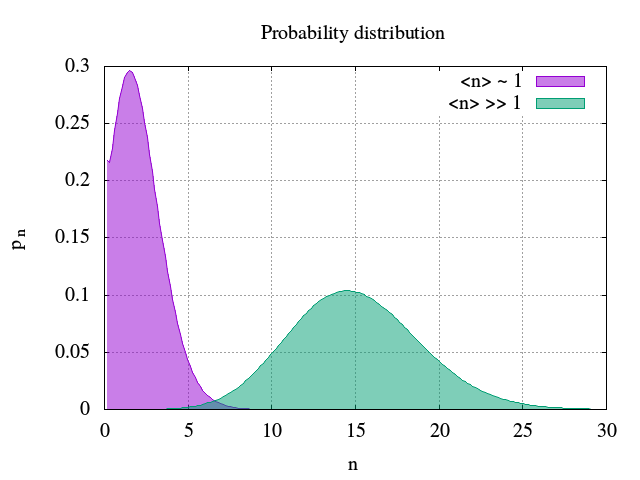
\includegraphics[width=0.7\linewidth]{fig/L2/2_1}
	\caption{Probability distribution for coherent state}
	\label{fig:2_1}
\end{figure}

\subsection{Orthogonality}

Are coherent states orthogonal or not? Lets find out:
\begin{equation}
	\braket{\alpha'}{\alpha} = e^{- \left|\alpha\right|^2/2} e^{- \left|\alpha'\right|^2/2} \sum \frac{( \accentset{\ast}{\alpha}' )^n \alpha^n}{n!} = e^{-\frac{1}{2} \left|\alpha\right|^2} e^{-\frac{1}{2} \left|\alpha'\right|^2 } e^{\accentset{\ast}{\alpha}' \alpha} \neq 0,
\end{equation}
\begin{equation}
	\left|\braket{\alpha'}{\alpha}\right|^2 = e^{- \left| \alpha - \alpha' \right|^2}.
\end{equation}



%\begin{testexample}[If you really want, you can consider coherent states as orthogonal ones!]
	\textcolor{red}{(UNCOMMENT THIS LATER! (see source))}
	\begin{equation}
	\begin{matrix}
	\ket{\alpha} &=& \ket{3+4i} \\
	\ket{\alpha'} &=& \ket{4+3i} \\
	\end{matrix}
	\quad \to \quad \left|\braket{\alpha'}{\alpha}\right|^2 = e^{-2} \approx 0.1
	\end{equation}
	\begin{equation}
	\begin{matrix}
	\ket{\alpha} &=& \ket{3+4i} \\
	\ket{\alpha'} &=& \ket{-4-3i} \\
	\end{matrix}
	\quad \to \quad \left|\braket{\alpha'}{\alpha}\right|^2  = e^{-98}.
	\end{equation}
	This is a VERY small value!
%\end{testexample}

Let the reader check the fullness of coherent states. In other words needless to show that
\begin{equation}
	\mathbb{1} = \frac{1}{\pi} \int \limits_{\mathbb{C}} d^2 \alpha \ket{\alpha} \bra{\alpha}.
\end{equation}
\textit{Hint:} for Fock states $\sum_{n=0}^{\infty} \ket{n} \bra{n} = 1$.\\
\textit{Remark:} actually coherent states have the property of overfullness in the sense these states form a basis,  {\textcolor{red}{ but not orthogonal,  }} and one may be expressed with the others.

Consider the following singlemode field. So this
\begin{equation}
	\hat{\vec{E}} = \sum_{\vec{k},s} \varepsilon_{\vec{k}s} \left( \hat{a}_{\vec{k}s} \vec{e}_{\vec{k}s} e^{i \vec{k} \vec{r} - i \omega_{\vec{k}}t} + \text{ e. c.} \right)
\end{equation}
will be simplified to
\begin{equation}
	\hat{\vec{E}} = \varepsilon \left( \hat{a} \vec{e} e^{i \vec{k} \vec{r} - \omega t} + \text{ e. c.}\right).
\end{equation}
Mean value 
\begin{equation}
	\vec{E} = \bra{\alpha} \hat{\vec{E}} \ket{\alpha} = \varepsilon \alpha \vec{e} e^{i \vec{k} \vec{r} - \omega t} + \text{ c. c.} \myeq \vec{E}_+(\vec{r},t) + \vec{E}_-(\vec{r},t).
\end{equation}
The amplitude is defined by $\alpha$:
\begin{equation}
	\vec{E}_+ = E_+ \vec{e} e^{i \vec{k} \vec{r} - \omega t}, \qquad E_+ = \alpha \varepsilon, \qquad \varepsilon = \sqrt{\frac{2 \pi \hbar}{V \omega}}.
\end{equation}
The intensity is proportional to
\begin{equation}
	I_+ \propto \left|E_+\right|^2 = \varepsilon^2 \left|\alpha\right|^2 = \varepsilon^2 \overline{n}.
\end{equation}
From here it is clear that $\varepsilon^2$ stands for the square of electric field amplitude per one photon. Often it is convenient to pick out a phase
\begin{equation}
	E_+ = \varepsilon \left|\alpha\right| e^{i \varphi}.
\end{equation}

Another property of coherent states. Since 
\begin{equation}
	\hat{a} \ket{\alpha} = \alpha \ket{\alpha},
\end{equation}
then number of photons in the system does not change!


\subsection{Fluctuations}

Let look at Fock states again. To draw a phase plane we need to remember that
\begin{equation}
	\hat{p} = i \sqrt{\frac{\hbar \omega}{2}} \left( \hat{a}^{\dagger} - \hat{a} \right), \qquad \hat{q} = \sqrt{\frac{\hbar}{2 \omega}}\left( \hat{a}^{\dagger} + \hat{a} \right).
\end{equation}
To find fluctuations let us compute
\begin{equation}
	\overline{p} = \bra{n} \hat{p} \ket{n} = 0, \qquad \overline{q} = \bra{n} \hat{q} \ket{n} = 0
\end{equation}
and
\begin{eqnarray}
	\overline{p^2} = \bra{n} \hat{p}^2 \ket{n} = \frac{\hbar \omega}{2} \left( 2n+1 \right), \\
	\overline{q^2} = \bra{n} \hat{q}^2 \ket{n} = \frac{\hbar}{2 \omega} \left( 2n+1 \right).
\end{eqnarray}
So we have
\begin{equation}
	\Delta p = \sqrt{\overline{p^2} - \overline{p}^2} = \sqrt{\frac{\hbar \omega}{2}} \sqrt{\left( 2n+1 \right)}, 
\end{equation}
\begin{equation}
	\Delta q = \sqrt{\overline{q^2} - \overline{q}^2} = \sqrt{\frac{\hbar }{2\omega}} \sqrt{\left( 2n+1 \right)}.
\end{equation}
Now we can the uncertainty principle as following
\begin{equation}
	\Delta p \Delta q = \frac{\hbar}{2} \left(2n+1\right).
\end{equation}

\begin{figure}
	\centering
	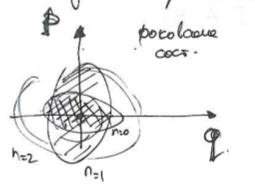
\includegraphics[width=0.4\linewidth]{fig/L2/fluc}
	\caption{Fluctuations of the Fock states}
	\label{fig:fluc}
\end{figure}

Now let us find the thing for coherent states:
\begin{equation}
	\overline{p} = \bra{\alpha} \hat{p} \ket{\alpha} = i \sqrt{\frac{\hbar \omega}{2}} \left( \alpha^* - \alpha \right) = 2 \sqrt{\frac{\hbar \omega}{2}} \Im \left\{ \alpha \right\},
\end{equation}
\begin{equation}
	\overline{q} = 2 \sqrt{\frac{\hbar }{2\omega}} \Re \left\{\alpha \right\},
\end{equation}
\begin{equation}
	\overline{p^2} = - \frac{\hbar \omega}{2} \bra{\alpha} \hat{a}^{\dagger 2} - \hat{a}^{\dagger} \hat{a} - \hat{a} \hat{a}^{\dagger} + \hat{a}^2  \ket{\alpha} = \frac{\hbar \omega}{2} \left( 4 \Im \left\{ \alpha \right\} + 1\right),
\end{equation}
\begin{equation}
	\overline{q^2} = \frac{\hbar}{2 \omega} \left( 4 \Re \left\{ \alpha \right\} + 1\right).
\end{equation}
Then
\begin{equation}
	\Delta p_{\alpha} = \sqrt{\frac{\hbar \omega}{2} \left[ 4 \Im \left\{ \alpha \right\} + 1 - 4 \Im \left\{ \alpha \right\} \right]^{1/2}} = \frac{\hbar \omega}{2}, \qquad \Delta q_{\alpha} = \frac{\hbar}{2 \omega}.
\end{equation}
The uncertainty relation will be
\begin{equation}
	\boxed{\Delta p_{\alpha} \Delta q_{\alpha} = \frac{\hbar}{2} \quad \slashed{\sim} \quad  \alpha.}
\end{equation}
Here we see that $\Delta p_{\alpha} \Delta q_{\alpha}$ relation does not depend on $\alpha$!
